\documentclass{article}
\usepackage{graphicx}
\graphicspath{ {images/} }
\usepackage[utf8]{inputenc}
\usepackage{listings}

\title{Programa 3 - Automata Finito Autodeterministico}
\author{Leon Tejeda 2CM5}
\date{Octubre 2020}

\begin{document}
\maketitle
\begin{flushleft}
Se nos encargo un programa que encontrara el n-esimo numero primo

INTRODUCCION:

Que es un automata:	Un autómata es un modelo matemático para una máquina de estado finito, en el que dada una entrada de símbolos, "salta" mediante una serie de estados de acuerdo a una función de transición (que puede ser expresada como una tabla). Esta función 					de transición indica a qué estado cambiar dados el estado actual y el símbolo leído.

Que son las palabras reservadas:	Las palabras reservadas en programación, o palabras clave, tienen un significado especial para el compilador de cualquier lenguaje de programación.

						Estas palabras pueden identificar los tipos de datos que se pueden usar, además de la diferentes rutinas de programación que permite cada lenguaje.

Palabras reservadas utilizadas de ANSI-C:
\begin{tabular}{c c}
auto		&	int \\
break		&	long \\
case		&	register \\
char		&	return \\
const		&	short \\
continue	&	signed \\
default	&	sizeof \\
do		&	static \\
double	&	struct \\
else		&	switch \\
enum		&	typedef \\
extern	&	union \\
float		&	unsigned \\
for		&	void \\
goto		&	volatile \\
if		&	while \\
\end{tabular} 

PLANTEAMIENTO DEL PROBLEMA:

Programar el autómata finito determinístico que reconozca todas las palabras reservadas del lenguaje ANSI C.

1. El programa deberá de leer un código (archivo) cualquiera.

2. El autómata deberá de identificar cada palabra reservada, contarlas y al final deberá decir cuántas encontró de cada una de ellas.

3. En un archivo imprimir la evaluación del autómata por cada carácter que lea y cambio de estado, es decir, toda la historia del proceso.

4. En otro archivo enumerar y contar cuántas palabras reservadas fueron encontradas.

5. Tener una opción para ver el autómata, es decir, hay que graficarlo.


IMPLEMENTACION:

Se aplicaron if's anidados, cada uno con su repectivo else para no tener problemas

Se implemento una lista que tuviera todas la palabras y las veces que aparecio en el archivo

Para el grafo se usaron librerias defautlt e python en donde se nos permitia unir los nodos con vertices e imprimirlo gracias a la libreria de matplotlib


Codigo:

\begin{lstlisting}

import networkx as nx
import matplotlib.pyplot as plt

def grafo(palabras):
    G=nx.Graph()
    
    #estado 0
    edge = ("0", "A")
    G.add_edge(*edge)
    edge = ("0", "B")
    G.add_edge(*edge)
    edge = ("0", "C")
    G.add_edge(*edge)
    edge = ("0", "D")
    G.add_edge(*edge)
    edge = ("0", "E")
    G.add_edge(*edge)
    edge = ("0", "F")
    G.add_edge(*edge)
    edge = ("0", "G")
    G.add_edge(*edge)
    edge = ("0", "I")
    G.add_edge(*edge)
    edge = ("0", "L")
    G.add_edge(*edge)
    edge = ("0", "R")
    G.add_edge(*edge)
    edge = ("0", "S")
    G.add_edge(*edge)
    edge = ("0", "T")
    G.add_edge(*edge)
    edge = ("0", "U")
    G.add_edge(*edge)
    edge = ("0", "V")
    G.add_edge(*edge)
    edge = ("0", "W")
    G.add_edge(*edge)

    #auto 1
    edge = ("A", "u1")
    G.add_edge(*edge)
    edge = ("u1", "t1")
    G.add_edge(*edge)
    edge = ("t1", "o1")
    G.add_edge(*edge)
    
    #break 2
    edge = ("B", "r2")
    G.add_edge(*edge)
    edge = ("r2", "e2")
    G.add_edge(*edge)
    edge = ("e2", "a2")
    G.add_edge(*edge)
    edge = ("a2", "k2")
    G.add_edge(*edge)
    
    #case 3
    edge = ("C", "a3")
    G.add_edge(*edge)
    edge = ("a3", "s3")
    G.add_edge(*edge)
    edge = ("s3", "e3")
    G.add_edge(*edge)
    
    #char 4
    edge = ("C", "h4")
    G.add_edge(*edge)
    edge = ("h4", "a4")
    G.add_edge(*edge)
    edge = ("a4", "r4")
    G.add_edge(*edge)
    
    #const 5
    edge = ("C", "o5")
    G.add_edge(*edge)
    edge = ("o5", "n5")
    G.add_edge(*edge)
    edge = ("n5", "s5")
    G.add_edge(*edge)
    edge = ("s5", "t5")
    G.add_edge(*edge)
    
    #continue 6
    edge = ("n5", "t6")
    G.add_edge(*edge)
    edge = ("t6", "i6")
    G.add_edge(*edge)
    edge = ("i6", "n6")
    G.add_edge(*edge)
    edge = ("n6", "u6")
    G.add_edge(*edge)
    edge = ("u6", "e6")
    G.add_edge(*edge)
    
    #default 7
    edge = ("D", "e7")
    G.add_edge(*edge)
    edge = ("e7", "f7")
    G.add_edge(*edge)
    edge = ("f7", "a7")
    G.add_edge(*edge)
    edge = ("a7", "u7")
    G.add_edge(*edge)
    edge = ("u7", "l7")
    G.add_edge(*edge)
    edge = ("l7", "t7")
    G.add_edge(*edge)
    
    #do 8
    edge = ("D", "o8")
    G.add_edge(*edge)
    
    #double 9
    edge = ("D", "o9")
    G.add_edge(*edge)
    edge = ("o9", "u9")
    G.add_edge(*edge)
    edge = ("u9", "b9")
    G.add_edge(*edge)
    edge = ("b9", "l9")
    G.add_edge(*edge)
    edge = ("l9", "e9")
    G.add_edge(*edge)
    
    #else 10
    edge = ("E", "l10")
    G.add_edge(*edge)
    edge = ("l10", "s10")
    G.add_edge(*edge)
    edge = ("s10", "e10")
    G.add_edge(*edge)
    
    #enum 11
    edge = ("E", "n11")
    G.add_edge(*edge)
    edge = ("n11", "u11")
    G.add_edge(*edge)
    edge = ("u11", "m11")
    G.add_edge(*edge)
    
    #extern 12
    edge = ("E", "x12")
    G.add_edge(*edge)
    edge = ("x12", "e12")
    G.add_edge(*edge)
    edge = ("e12", "r12")
    G.add_edge(*edge)
    edge = ("r12", "n12")
    G.add_edge(*edge)
    
    #float 13
    edge = ("F", "l13")
    G.add_edge(*edge)
    edge = ("l13", "o13")
    G.add_edge(*edge)
    edge = ("o13", "a13")
    G.add_edge(*edge)
    edge = ("a13", "t13")
    G.add_edge(*edge)
    
    #for 14
    edge = ("F", "o14")
    G.add_edge(*edge)
    edge = ("o14", "r14")
    G.add_edge(*edge)
    
    #goto 15
    edge = ("G", "o15")
    G.add_edge(*edge)
    edge = ("o15", "t15")
    G.add_edge(*edge)
    edge = ("t15", "o15")
    G.add_edge(*edge)
    
    #if 16
    edge = ("I", "f16")
    G.add_edge(*edge)
    
    #int 17
    edge = ("I", "n17")
    G.add_edge(*edge)
    edge = ("n17", "t17")
    G.add_edge(*edge)
    
    #long 18
    edge = ("L", "o18")
    G.add_edge(*edge)
    edge = ("o18", "n18")
    G.add_edge(*edge)
    edge = ("n18", "g18")
    G.add_edge(*edge)
    
    #register 19
    edge = ("R", "e19")
    G.add_edge(*edge)
    edge = ("e19", "g19")
    G.add_edge(*edge)
    edge = ("g19", "i19")
    G.add_edge(*edge)
    edge = ("i19", "s19")
    G.add_edge(*edge)
    edge = ("s19", "t19")
    G.add_edge(*edge)
    edge = ("t19", "e19")
    G.add_edge(*edge)
    edge = ("e19", "r19")
    G.add_edge(*edge)

    #return 20
    edge = ("e19", "t20")
    G.add_edge(*edge)
    edge = ("t20", "u20")
    G.add_edge(*edge)
    edge = ("u20", "r20")
    G.add_edge(*edge)
    edge = ("r20", "n20")
    G.add_edge(*edge)
    
    #short 21
    edge = ("S", "h21")
    G.add_edge(*edge)
    edge = ("h21", "o21")
    G.add_edge(*edge)
    edge = ("o21", "r21")
    G.add_edge(*edge)
    edge = ("r21", "t21")
    G.add_edge(*edge)
    
    #signed 22
    edge = ("S", "i22")
    G.add_edge(*edge)
    edge = ("i22", "g22")
    G.add_edge(*edge)
    edge = ("g22", "n22")
    G.add_edge(*edge)
    edge = ("n22", "e22")
    G.add_edge(*edge)
    edge = ("e22", "d22")
    G.add_edge(*edge)
    
    #sizeof 23
    edge = ("i22", "z23")
    G.add_edge(*edge)
    edge = ("z23", "e23")
    G.add_edge(*edge)
    edge = ("e23", "o23")
    G.add_edge(*edge)
    edge = ("o23", "f23")
    G.add_edge(*edge)
    
    #static 24
    edge = ("S", "t24")
    G.add_edge(*edge)
    edge = ("t24", "t24")
    G.add_edge(*edge)
    edge = ("t24", "a24")
    G.add_edge(*edge)
    edge = ("a24", "t24")
    G.add_edge(*edge)
    edge = ("t24", "i24")
    G.add_edge(*edge)
    edge = ("i24", "c24")
    G.add_edge(*edge)
    
    #struct 25
    edge = ("t24", "r25")
    G.add_edge(*edge)
    edge = ("r25", "u25")
    G.add_edge(*edge)
    edge = ("u25", "c25")
    G.add_edge(*edge)
    edge = ("c25", "t25")
    G.add_edge(*edge)
    
    #switch 26
    edge = ("S", "w26")
    G.add_edge(*edge)
    edge = ("w26", "i26")
    G.add_edge(*edge)
    edge = ("i26", "t26")
    G.add_edge(*edge)
    edge = ("t26", "c26")
    G.add_edge(*edge)
    edge = ("c26", "h26")
    G.add_edge(*edge)
    
    #ypeddef 27
    edge = ("T", "y27")
    G.add_edge(*edge)
    edge = ("y27", "p27")
    G.add_edge(*edge)
    edge = ("p27", "e27")
    G.add_edge(*edge)
    edge = ("e27", "d27")
    G.add_edge(*edge)
    edge = ("d27", "e27")
    G.add_edge(*edge)
    edge = ("e27", "f27")
    G.add_edge(*edge)
    
    #union 28
    edge = ("U", "n28")
    G.add_edge(*edge)
    edge = ("n28", "i28")
    G.add_edge(*edge)
    edge = ("i28", "o28")
    G.add_edge(*edge)
    edge = ("o28", "n28")
    G.add_edge(*edge)
    
    #unsigned 29
    edge = ("n28", "s29")
    G.add_edge(*edge)
    edge = ("s29", "i29")
    G.add_edge(*edge)
    edge = ("i29", "g29")
    G.add_edge(*edge)
    edge = ("g29", "n29")
    G.add_edge(*edge)
    edge = ("n29", "e29")
    G.add_edge(*edge)
    edge = ("e29", "d29")
    G.add_edge(*edge)

    #void 30
    edge = ("V", "o30")
    G.add_edge(*edge)
    edge = ("o30", "i30")
    G.add_edge(*edge)
    edge = ("i30", "d30")
    G.add_edge(*edge)
    
    #volatile 31
    edge = ("o30", "l31")
    G.add_edge(*edge)
    edge = ("l31", "a31")
    G.add_edge(*edge)
    edge = ("a31", "t31")
    G.add_edge(*edge)
    edge = ("t31", "i31")
    G.add_edge(*edge)
    edge = ("i31", "l31")
    G.add_edge(*edge)
    edge = ("l31", "e31")
    G.add_edge(*edge)
    
    #while 32
    edge = ("W", "h32")
    G.add_edge(*edge)
    edge = ("h32", "i32")
    G.add_edge(*edge)
    edge = ("i32", "l32")
    G.add_edge(*edge)
    edge = ("l32", "e32")
    G.add_edge(*edge)
    
    #print("Nodes of graph: ")
    #print(G.nodes())
    #print("Edges of graph: ")
    #print(G.edges())

    nx.draw(G)
    plt.savefig("Programa3-Grafo.png") # save as png
    plt.show() # display


def automata_archivo(caracter, aceptado, estado, palabra):
    automata = open("Programa3_EstadosDelAutomata.txt", "a")
        
    if caracter.isalpha() != True:
        cadena = "f(q144, Simbolo) -> Cadena No Valida"
        automata.write(cadena)
        automata.write("\n")
            
    
    elif aceptado == 0:
        cadena = "f(q" + str(estado) + ", " + caracter + ") -> q" + str(estado + 1) + " "
        automata.write(cadena)
    
    
    elif aceptado == False:
        cadena = "f(q" + str(estado) + ", " + caracter + ") -> Cadena No Valida"
        automata.write(cadena)
        automata.write("\n")
        
    else:
        cadena = "f(q" + str(estado) + ", " + caracter + ") -> q" + str(estado + 1) + " Acepta Cadena: " + palabra
        automata.write(cadena)
        automata.write("\n")
    
    automata.close()
    
    
def palabras_encontradas(lista):
    total = 0
    
    archivo = open("Programa3_PalabrasEncontradas.txt", "w")
    
    for i in range(0, 64):    
        if i % 2 != 0:
            archivo.write(str(lista[i]))
            total = int(lista[i]) + total
            archivo.write("\n")
            
        else:
            archivo.write(str(lista[i]))
            archivo.write(": ")
    
    archivo.write("Total de Palabras Econtradas: ")
    archivo.write(str(total))        
    archivo.close()


def borrar_archivos():
    archivo = open("Programa3_EstadosDelAutomata.txt", "w")
    archivo.close()


def palabras_ansic():
    palabras = []
    
    for i in range(0, 64):
        palabras.insert(i, 0)
    
    palabras[0] = 'auto'
    palabras[2] = 'break'
    palabras[4] = 'case'
    palabras[6] = 'char'
    palabras[8] = 'const'
    palabras[10] = 'continue'
    palabras[12] = 'default'
    palabras[14] = 'do'
    palabras[16] = 'double'
    palabras[18] = 'else'
    palabras[20] = 'enum'
    palabras[22] = 'extern'
    palabras[24] =  'float'
    palabras[26] = 'for'
    palabras[28] = 'goto'
    palabras[30] = 'if'
    palabras[32] = 'int'
    palabras[34] = 'long'
    palabras[36] = 'register'
    palabras[38] = 'return'
    palabras[40] = 'short'
    palabras[42] = 'signed'
    palabras[44] = 'sizeof'
    palabras[46] = 'static'
    palabras[48] = 'struct'
    palabras[50] = 'switch'
    palabras[52] = 'typedef'
    palabras[54] = 'union'
    palabras[56] = 'unsigned'
    palabras[58] = 'void'
    palabras[60] = 'volatile'
    palabras[62] =  'while'
        
    return palabras


def leer_codigo():
    archivo = open("Programa3_CodigoC-ANSI.txt", "r")
    palabras = palabras_ansic()
    
    
    for caracter in archivo:
        for i in range (0, len(caracter)):
            estado = 0
            aceptado = 0
            cadena = 0

            #auto
            if caracter[i] == 'a':
                cadena = caracter[i]
                i = i + 1
                estado = 1
                automata_archivo(cadena, aceptado, estado, palabras[0])
                
                if caracter[i] == 'u':
                    cadena = caracter [i]
                    i = i + 1
                    estado = 2
                    automata_archivo(cadena, aceptado, estado, palabras[0])   
                    
                    if caracter[i] == 't':
                        cadena = caracter [i]
                        i = i + 1
                        estado = 3
                        automata_archivo(cadena, aceptado, estado, palabras[0])
                        
                        if caracter[i] == 'o':
                            cadena = caracter[i]
                            palabras[1] = palabras[1] + 1
                            estado = 4
                            aceptado = True
                            automata_archivo(cadena, aceptado, estado, palabras[0])
                            
                        else:
                            cadena = caracter [i]
                            aceptado = False
                            automata_archivo(cadena, aceptado, estado, palabras[0])
                            
                    else:
                        cadena = caracter [i]
                        aceptado = False
                        automata_archivo(cadena, aceptado, estado, palabras[0])
                
                else:
                    cadena = caracter [i]
                    aceptado = False
                    automata_archivo(cadena, aceptado, estado, palabras[0])
                            
            
            #break
            elif caracter[i] == 'b':
                cadena = caracter[i]
                i = i + 1
                estado = 5
                automata_archivo(cadena, aceptado, estado, palabras[2])
                
                if caracter[i] == 'r':
                    cadena = caracter [i]
                    i = i + 1
                    estado = 6
                    automata_archivo(cadena, aceptado, estado, palabras[2])              
                    
                    if caracter[i] == 'e':
                        cadena = caracter [i]
                        i = i + 1
                        estado = 7
                        automata_archivo(cadena, aceptado, estado, palabras[2])
                        
                        if caracter[i] == 'a':
                            cadena = caracter [i]
                            i = i + 1
                            estado = 8
                            automata_archivo(cadena, aceptado, estado, palabras[2])
                            
                            if caracter[i] == 'k':
                                cadena = caracter[i]
                                palabras[3] = palabras[3] + 1
                                estado = 9
                                aceptado = True
                                automata_archivo(cadena, aceptado, estado, palabras[2])
                                
                            else:
                                cadena = caracter [i]
                                aceptado = False
                                automata_archivo(cadena, aceptado, estado, palabras[2])
                        
                        else:
                            cadena = caracter [i]
                            aceptado = False
                            automata_archivo(cadena, aceptado, estado, palabras[2])
                            
                    else:
                        cadena = caracter [i]
                        aceptado = False
                        automata_archivo(cadena, aceptado, estado, palabras[2])
                    
                else:
                    cadena = caracter [i]
                    aceptado = False
                    automata_archivo(cadena, aceptado, estado, palabras[2])
                    
            #c
            elif caracter[i] == 'c':
                cadena = caracter[i]
                i = i + 1
                estado = 10
                automata_archivo(cadena, aceptado, estado, palabras[4])
                
                #case
                if caracter[i] == 'a':
                    cadena = caracter [i]
                    i = i + 1
                    estado = 11
                    automata_archivo(cadena, aceptado, estado, palabras[4])   
                    
                    if caracter[i] == 's':
                        cadena = caracter [i]
                        i = i + 1
                        estado = 12
                        automata_archivo(cadena, aceptado, estado, palabras[4])
                        
                        if caracter[i] == 'e':
                            cadena = caracter[i]
                            palabras[5] = palabras[5] + 1
                            estado = 13
                            aceptado = True
                            automata_archivo(cadena, aceptado, estado, palabras[4])
                            
                        else:
                            cadena = caracter [i]
                            aceptado = False
                            automata_archivo(cadena, aceptado, estado, palabras[4])
                            
                    else:
                        cadena = caracter [i]
                        aceptado = False
                        automata_archivo(cadena, aceptado, estado, palabras[4])
                
                else:
                    cadena = caracter [i]
                    aceptado = False
                    automata_archivo(cadena, aceptado, estado, palabras[4])
                    
                #char    
                if caracter[i] == 'h':
                    cadena = caracter [i]
                    i = i + 1
                    estado = 14
                    automata_archivo(cadena, aceptado, estado, palabras[6])   
                    
                    if caracter[i] == 'a':
                        cadena = caracter [i]
                        i = i + 1
                        estado = 15
                        automata_archivo(cadena, aceptado, estado, palabras[6])
                        
                        if caracter[i] == 'r':
                            cadena = caracter[i]
                            palabras[7] = palabras[7] + 1
                            estado = 16
                            aceptado = True
                            automata_archivo(cadena, aceptado, estado, palabras[6])
                            
                        else:
                            cadena = caracter [i]
                            aceptado = False
                            automata_archivo(cadena, aceptado, estado, palabras[6])
                            
                    else:
                        cadena = caracter [i]
                        aceptado = False
                        automata_archivo(cadena, aceptado, estado, palabras[6])
                
                else:
                    cadena = caracter [i]
                    aceptado = False
                    automata_archivo(cadena, aceptado, estado, palabras[6])
                    
                
                
                if caracter[i] == 'o':
                    cadena = caracter[i]
                    i = i + 1
                    estado = 17
                    automata_archivo(cadena, aceptado, estado, palabras[8])
                    
                    if caracter[i] == 'n':
                        cadena = caracter [i]
                        i = i + 1
                        estado = 18
                        automata_archivo(cadena, aceptado, estado, palabras[8])   
                        
                        #const
                        if caracter[i] == 's':
                            cadena = caracter [i]
                            i = i + 1
                            estado = 19
                            automata_archivo(cadena, aceptado, estado, palabras[8])
                            
                            if caracter[i] == 't':
                                cadena = caracter[i]
                                palabras[9] = palabras[9] + 1
                                estado = 20
                                aceptado = True
                                automata_archivo(cadena, aceptado, estado, palabras[8])
                                
                            else:
                                cadena = caracter [i]
                                aceptado = False
                                automata_archivo(cadena, aceptado, estado, palabras[8])
                                
                        #continue
                        elif caracter[i] == 't':
                            cadena = caracter[i]
                            i = i + 1
                            estado = 21
                            automata_archivo(cadena, aceptado, estado, palabras[10])
                            
                            if caracter[i] == 'i':
                                cadena = caracter[i]
                                i = i + 1
                                estado = 22
                                automata_archivo(cadena, aceptado, estado, palabras[10])
                                
                                if caracter[i] == 'n':
                                    cadena = caracter[i]
                                    i = i + 1
                                    estado = 23
                                    automata_archivo(cadena, aceptado, estado, palabras[10])
                                    
                                    if caracter[i] == 'u':
                                        cadena = caracter[i]
                                        i = i + 1
                                        estado = 24
                                        automata_archivo(cadena, aceptado, estado, palabras[10])
                                        
                                        if caracter[i] == 'e':
                                            cadena = caracter[i]
                                            palabras[11] = palabras[11] + 1
                                            estado = 25
                                            aceptado = True
                                            automata_archivo(cadena, aceptado, estado, palabras[10])
                                            
                                        else:
                                            cadena = caracter [i]
                                            aceptado = False
                                            automata_archivo(cadena, aceptado, estado, palabras[10])
                                    
                                    else:
                                        cadena = caracter [i]
                                        aceptado = False
                                        automata_archivo(cadena, aceptado, estado, palabras[10])
                                        
                                else:
                                    cadena = caracter [i]
                                    aceptado = False
                                    automata_archivo(cadena, aceptado, estado, palabras[10])
                                    
                            else:
                                cadena = caracter [i]
                                aceptado = False
                                automata_archivo(cadena, aceptado, estado, palabras[10])
                        
                        
                        else:
                            cadena = caracter [i]
                            aceptado = False
                            automata_archivo(cadena, aceptado, estado, palabras[8])
                    
                    else:
                        cadena = caracter [i]
                        aceptado = False
                        automata_archivo(cadena, aceptado, estado, palabras[8])
                else:
                    cadena = caracter [i]
                    aceptado = False
                    automata_archivo(cadena, aceptado, estado, palabras[8])
                        
            #d
            elif caracter[i] == 'd':
                cadena = caracter[i]
                i = i + 1
                estado = 26
                automata_archivo(cadena, aceptado, estado, palabras[12])
                
                #default
                if caracter[i] == 'e':
                    cadena = caracter[i]
                    i = i + 1
                    estado = 27
                    automata_archivo(cadena, aceptado, estado, palabras[12])
                    
                    if caracter[i] == 'f':
                        cadena = caracter[i]
                        i = i + 1
                        estado = 28
                        automata_archivo(cadena, aceptado, estado, palabras[12])
                        
                        if caracter[i] == 'a':
                            cadena = caracter[i]
                            i = i + 1
                            estado = 29
                            automata_archivo(cadena, aceptado, estado, palabras[12])
                            
                            if caracter[i] == 'u':
                                cadena = caracter[i]
                                i = i + 1
                                estado = 30
                                automata_archivo(cadena, aceptado, estado, palabras[12])
                                
                                if caracter[i] == 'l':
                                    cadena = caracter[i]
                                    i = i + 1
                                    estado = 31
                                    automata_archivo(cadena, aceptado, estado, palabras[12])
                                    
                                    if caracter[i] == 't':
                                        cadena = caracter[i]
                                        palabras[13] = palabras[13] + 1
                                        estado = 32
                                        aceptado = True
                                        automata_archivo(cadena, aceptado, estado, palabras[12])
                                        
                                    else:
                                        cadena = caracter [i]
                                        aceptado = False
                                        automata_archivo(cadena, aceptado, estado, palabras[12])
                                        
                                else:
                                    cadena = caracter [i]
                                    aceptado = False
                                    automata_archivo(cadena, aceptado, estado, palabras[12])
                                    
                            else:
                                cadena = caracter [i]
                                aceptado = False
                                automata_archivo(cadena, aceptado, estado, palabras[12])
                                
                        else:
                            cadena = caracter [i]
                            aceptado = False
                            automata_archivo(cadena, aceptado, estado, palabras[12])
                            
                    else:
                        cadena = caracter [i]
                        aceptado = False
                        automata_archivo(cadena, aceptado, estado, palabras[12])
                        
                #do y double
                elif caracter[i] == 'o':
                    cadena = caracter[i]
                    i = i + 1
                    estado = 33
                    automata_archivo(cadena, aceptado, estado, palabras[14])
                    
                    #do
                    if caracter[i].isalpha() != True:
                        palabras[15] = palabras[15] + 1
                        aceptado = True
                        automata_archivo(cadena, aceptado, estado, palabras[14])
                        
                    #double
                    elif caracter[i] == 'u':
                        cadena = caracter[i]
                        i = i + 1
                        estado = 34
                        automata_archivo(cadena, aceptado, estado, palabras[16])
                    

                        if caracter[i] == 'b':
                            cadena = caracter[i]
                            i = i + 1
                            estado = 35
                            automata_archivo(cadena, aceptado, estado, palabras[16])
                            
                            if caracter[i] == 'l':
                                cadena = caracter[i]
                                i = i + 1
                                estado = 36
                                automata_archivo(cadena, aceptado, estado, palabras[16])
                                
                                if caracter[i] == 'e':
                                    cadena = caracter[i]
                                    palabras[17] = palabras[17] + 1
                                    estado = 37
                                    aceptado = True
                                    automata_archivo(cadena, aceptado, estado, palabras[16])
                                    
                                else:
                                    cadena = caracter [i]
                                    aceptado = False
                                    automata_archivo(cadena, aceptado, estado, palabras[16])
                                    
                            else:
                                cadena = caracter [i]
                                aceptado = False
                                automata_archivo(cadena, aceptado, estado, palabras[16])
                                
                        else:
                            cadena = caracter [i]
                            aceptado = False
                            automata_archivo(cadena, aceptado, estado, palabras[16])
                            
                    else:
                        cadena = caracter [i]
                        aceptado = False
                        automata_archivo(cadena, aceptado, estado, palabras[14])
                
                
                else:
                    cadena = caracter [i]
                    aceptado = False
                    automata_archivo(cadena, aceptado, estado, palabras[12])
                    
            
            #e
            elif caracter[i] == 'e':
                cadena = caracter[i]
                i = i + 1
                estado = 38
                automata_archivo(cadena, aceptado, estado, palabras[18])
                
                #else
                if caracter[i] == 'l':
                    cadena = caracter [i]
                    i = i + 1
                    estado = 39
                    automata_archivo(cadena, aceptado, estado, palabras[18])   
                    
                    if caracter[i] == 's':
                        cadena = caracter [i]
                        i = i + 1
                        estado = 40
                        automata_archivo(cadena, aceptado, estado, palabras[18])
                        
                        if caracter[i] == 'e':
                            cadena = caracter[i]
                            palabras[19] = palabras[19] + 1
                            estado = 41
                            aceptado = True
                            automata_archivo(cadena, aceptado, estado, palabras[18])
                            
                        else:
                            cadena = caracter [i]
                            aceptado = False
                            automata_archivo(cadena, aceptado, estado, palabras[18])
                            
                    else:
                        cadena = caracter [i]
                        aceptado = False
                        automata_archivo(cadena, aceptado, estado, palabras[18])
                        
                        
                #enum
                elif caracter[i] == 'n':
                    cadena = caracter [i]
                    i = i + 1
                    estado = 42
                    automata_archivo(cadena, aceptado, estado, palabras[20])   
                    
                    if caracter[i] == 'u':
                        cadena = caracter [i]
                        i = i + 1
                        estado = 43
                        automata_archivo(cadena, aceptado, estado, palabras[20])
                        
                        if caracter[i] == 'm':
                            cadena = caracter[i]
                            palabras[21] = palabras[21] + 1
                            estado = 44
                            aceptado = True
                            automata_archivo(cadena, aceptado, estado, palabras[20])
                            
                        else:
                            cadena = caracter [i]
                            aceptado = False
                            automata_archivo(cadena, aceptado, estado, palabras[20])
                            
                    else:
                        cadena = caracter [i]
                        aceptado = False
                        automata_archivo(cadena, aceptado, estado, palabras[20])
                                         
                
                #extern
                elif caracter[i] == 'x':
                    cadena = caracter[i]
                    i = i + 1
                    estado = 45
                    automata_archivo(cadena, aceptado, estado, palabras[22])
                    if caracter[i] == 't':
                        cadena = caracter [i]
                        i = i + 1
                        estado = 46
                        automata_archivo(cadena, aceptado, estado, palabras[22])              
                        
                        if caracter[i] == 'e':
                            cadena = caracter [i]
                            i = i + 1
                            estado = 47
                            automata_archivo(cadena, aceptado, estado, palabras[22])
                            
                            if caracter[i] == 'r':
                                cadena = caracter [i]
                                i = i + 1
                                estado = 48
                                automata_archivo(cadena, aceptado, estado, palabras[22])
                                
                                if caracter[i] == 'n':
                                    cadena = caracter[i]
                                    palabras[23] = palabras[23] + 1
                                    estado = 49
                                    aceptado = True
                                    automata_archivo(cadena, aceptado, estado, palabras[22])
                                    
                                else:
                                    cadena = caracter [i]
                                    aceptado = False
                                    automata_archivo(cadena, aceptado, estado, palabras[22])
                            
                            else:
                                cadena = caracter [i]
                                aceptado = False
                                automata_archivo(cadena, aceptado, estado, palabras[22])
                                
                        else:
                            cadena = caracter [i]
                            aceptado = False
                            automata_archivo(cadena, aceptado, estado, palabras[22])
                        
                    else:
                        cadena = caracter [i]
                        aceptado = False
                        automata_archivo(cadena, aceptado, estado, palabras[22])
                
                
                else:
                    cadena = caracter [i]
                    aceptado = False
                    automata_archivo(cadena, aceptado, estado, palabras[18])
            
            
            #f
            elif caracter[i] == 'f':
                cadena = caracter[i]
                i = i + 1
                estado = 51
                automata_archivo(cadena, aceptado, estado, palabras[24])
                
                #float
                if caracter[i] == 'l':
                    cadena = caracter[i]
                    i = i + 1
                    estado = 52
                    automata_archivo(cadena, aceptado, estado, palabras[24])
                    
                    if caracter[i] == 'o':
                        cadena = caracter [i]
                        i = i + 1
                        estado = 53
                        automata_archivo(cadena, aceptado, estado, palabras[24])   
                        
                        if caracter[i] == 'a':
                            cadena = caracter [i]
                            i = i + 1
                            estado = 54
                            automata_archivo(cadena, aceptado, estado, palabras[24])
                            
                            if caracter[i] == 't':
                                cadena = caracter[i]
                                palabras[25] = palabras[25] + 1
                                estado = 55
                                aceptado = True
                                automata_archivo(cadena, aceptado, estado, palabras[24])
                                
                            else:
                                cadena = caracter [i]
                                aceptado = False
                                automata_archivo(cadena, aceptado, estado, palabras[24])
                                
                        else:
                            cadena = caracter [i]
                            aceptado = False
                            automata_archivo(cadena, aceptado, estado, palabras[24])
                    
                    else:
                        cadena = caracter [i]
                        aceptado = False
                        automata_archivo(cadena, aceptado, estado, palabras[24])
                        
                #for
                elif caracter[i] == 'o':
                    cadena = caracter[i]
                    i = i + 1
                    estado = 56
                    automata_archivo(cadena, aceptado, estado, palabras[26])
                    
                    if caracter[i] == 'r':
                        cadena = caracter[i]
                        palabras[27] = palabras[27] + 1
                        estado = 57
                        aceptado = True
                        automata_archivo(cadena, aceptado, estado, palabras[26])
                                
                    else:
                        cadena = caracter [i]
                        aceptado = False
                        automata_archivo(cadena, aceptado, estado, palabras[26])
                                
                else:
                    cadena = caracter [i]
                    aceptado = False
                    automata_archivo(cadena, aceptado, estado, palabras[24])
                
                
            
            #goto
            elif caracter[i] == 'g':
                cadena = caracter[i]
                i = i + 1
                estado = 58
                automata_archivo(cadena, aceptado, estado, palabras[28])
                
                if caracter[i] == 'o':
                    cadena = caracter [i]
                    i = i + 1
                    estado = 59
                    automata_archivo(cadena, aceptado, estado, palabras[28])   
                    
                    if caracter[i] == 't':
                        cadena = caracter [i]
                        i = i + 1
                        estado = 60
                        automata_archivo(cadena, aceptado, estado, palabras[28])
                        
                        if caracter[i] == 'o':
                            cadena = caracter[i]
                            palabras[29] = palabras[29] + 1
                            estado = 61
                            aceptado = True
                            automata_archivo(cadena, aceptado, estado, palabras[28])
                            
                        else:
                            cadena = caracter [i]
                            aceptado = False
                            automata_archivo(cadena, aceptado, estado, palabras[28])
                            
                    else:
                        cadena = caracter [i]
                        aceptado = False
                        automata_archivo(cadena, aceptado, estado, palabras[28])
                
                else:
                    cadena = caracter [i]
                    aceptado = False
                    automata_archivo(cadena, aceptado, estado, palabras[28])
                
                
            #i
            elif caracter[i] == 'i':
                cadena = caracter [i]
                i = i + 1
                estado = 62
                automata_archivo(cadena, aceptado, estado, palabras[30])
                        
                #if
                if caracter[i] == 'f':
                    cadena = caracter[i]
                    palabras[31] = palabras[31] + 1
                    estado = 63
                    aceptado = True
                    automata_archivo(cadena, aceptado, estado, palabras[30])
                    
                    
                #int
                elif caracter[i] == 'n':
                    cadena = caracter [i]
                    i = i + 1
                    estado = 64
                    automata_archivo(cadena, aceptado, estado, palabras[32])
                        
                    if caracter[i] == 't':
                        cadena = caracter[i]
                        palabras[33] = palabras[33] + 1
                        estado = 65
                        aceptado = True
                        automata_archivo(cadena, aceptado, estado, palabras[32])
                            
                    else:
                        cadena = caracter [i]
                        aceptado = False
                        automata_archivo(cadena, aceptado, estado, palabras[32])
                            
                else:
                    cadena = caracter [i]
                    aceptado = False
                    automata_archivo(cadena, aceptado, estado, palabras[30])
                            
                   
            #long
            elif caracter[i] == 'l':
                cadena = caracter[i]
                i = i + 1
                estado = 66
                automata_archivo(cadena, aceptado, estado, palabras[34])
                
                if caracter[i] == 'o':
                    cadena = caracter [i]
                    i = i + 1
                    estado = 67
                    automata_archivo(cadena, aceptado, estado, palabras[34])   
                    
                    if caracter[i] == 'n':
                        cadena = caracter [i]
                        i = i + 1
                        estado = 68
                        automata_archivo(cadena, aceptado, estado, palabras[34])
                        
                        if caracter[i] == 'g':
                            cadena = caracter[i]
                            palabras[35] = palabras[35] + 1
                            estado = 69
                            aceptado = True
                            automata_archivo(cadena, aceptado, estado, palabras[34])
                            
                        else:
                            cadena = caracter [i]
                            aceptado = False
                            automata_archivo(cadena, aceptado, estado, palabras[34])
                            
                    else:
                        cadena = caracter [i]
                        aceptado = False
                        automata_archivo(cadena, aceptado, estado, palabras[34])
                
                else:
                    cadena = caracter [i]
                    aceptado = False
                    automata_archivo(cadena, aceptado, estado, palabras[34])
              
                
            
            #r
            elif caracter[i] == 'r':
                cadena = caracter[i]
                i = i + 1
                estado = 70
                automata_archivo(cadena, aceptado, estado, palabras[36])
                
                if caracter[i] == 'e':
                    cadena = caracter[i]
                    i = i + 1
                    estado = 71
                    automata_archivo(cadena, aceptado, estado, palabras[36])
                    
                    #register
                    if caracter[i] == 'g':
                        cadena = caracter[i]
                        i = i + 1
                        estado = 72
                        automata_archivo(cadena, aceptado, estado, palabras[36])
                        
                        if caracter[i] == 'i':
                            cadena = caracter[i]
                            i = i + 1
                            estado = 73
                            automata_archivo(cadena, aceptado, estado, palabras[36])
                            
                            if caracter[i] == 's':
                                cadena = caracter[i]
                                i = i + 1
                                estado = 74
                                automata_archivo(cadena, aceptado, estado, palabras[36])
                                
                                if caracter[i] == 't':
                                    cadena = caracter[i]
                                    i = i + 1
                                    estado = 75
                                    automata_archivo(cadena, aceptado, estado, palabras[36])
                                    
                                    if caracter[i] == 'e':
                                        cadena = caracter[i]
                                        i = i + 1
                                        estado = 76
                                        automata_archivo(cadena, aceptado, estado, palabras[36])
                                    
                                        if caracter[i] == 'r':
                                            cadena = caracter[i]
                                            palabras[37] = palabras[37] + 1
                                            estado = 77
                                            aceptado = True
                                            automata_archivo(cadena, aceptado, estado, palabras[36])
                                            
                                        else:
                                            cadena = caracter [i]
                                            aceptado = False
                                            automata_archivo(cadena, aceptado, estado, palabras[36])
                                    
                                    else:
                                        cadena = caracter [i]
                                        aceptado = False
                                        automata_archivo(cadena, aceptado, estado, palabras[36])
                                        
                                else:
                                    cadena = caracter [i]
                                    aceptado = False
                                    automata_archivo(cadena, aceptado, estado, palabras[36])
                                    
                            else:
                                cadena = caracter [i]
                                aceptado = False
                                automata_archivo(cadena, aceptado, estado, palabras[36])
                                
                        else:
                            cadena = caracter [i]
                            aceptado = False
                            automata_archivo(cadena, aceptado, estado, palabras[36])
                            
                            
                    #return
                    if caracter[i] == 't':
                        cadena = caracter [i]
                        i = i + 1
                        estado = 79
                        automata_archivo(cadena, aceptado, estado, palabras[38])              
                        
                        if caracter[i] == 'u':
                            cadena = caracter [i]
                            i = i + 1
                            estado = 80
                            automata_archivo(cadena, aceptado, estado, palabras[38])
                            
                            if caracter[i] == 'r':
                                cadena = caracter [i]
                                i = i + 1
                                estado = 81
                                automata_archivo(cadena, aceptado, estado, palabras[38])
                                
                                if caracter[i] == 'n':
                                    cadena = caracter[i]
                                    palabras[39] = palabras[39] + 1
                                    estado = 82
                                    aceptado = True
                                    automata_archivo(cadena, aceptado, estado, palabras[38])
                                    
                                else:
                                    cadena = caracter [i]
                                    aceptado = False
                                    automata_archivo(cadena, aceptado, estado, palabras[38])
                            
                            else:
                                cadena = caracter [i]
                                aceptado = False
                                automata_archivo(cadena, aceptado, estado, palabras[38])
                                
                        else:
                            cadena = caracter [i]
                            aceptado = False
                            automata_archivo(cadena, aceptado, estado, palabras[38])
                            
                    else:
                        cadena = caracter [i]
                        aceptado = False
                        automata_archivo(cadena, aceptado, estado, palabras[36])
                
                else:
                    cadena = caracter [i]
                    aceptado = False
                    automata_archivo(cadena, aceptado, estado, palabras[36])
                                        
            #s
            elif caracter[i] == 's':
                cadena = caracter[i]
                i = i + 1
                estado = 83
                automata_archivo(cadena, aceptado, estado, palabras[40])
                
                #short
                if caracter[i] == 'h':
                    cadena = caracter [i]
                    i = i + 1
                    estado = 84
                    automata_archivo(cadena, aceptado, estado, palabras[40])              
                    
                    if caracter[i] == 'o':
                        cadena = caracter [i]
                        i = i + 1
                        estado = 85
                        automata_archivo(cadena, aceptado, estado, palabras[40])
                        
                        if caracter[i] == 'r':
                            cadena = caracter [i]
                            i = i + 1
                            estado = 86
                            automata_archivo(cadena, aceptado, estado, palabras[40])
                            
                            if caracter[i] == 't':
                                cadena = caracter[i]
                                palabras[41] = palabras[41] + 1
                                estado = 87
                                aceptado = True
                                automata_archivo(cadena, aceptado, estado, palabras[40])
                                
                            else:
                                cadena = caracter [i]
                                aceptado = False
                                automata_archivo(cadena, aceptado, estado, palabras[40])
                        
                        else:
                            cadena = caracter [i]
                            aceptado = False
                            automata_archivo(cadena, aceptado, estado, palabras[40])
                            
                    else:
                        cadena = caracter [i]
                        aceptado = False
                        automata_archivo(cadena, aceptado, estado, palabras[40])
                        
                elif caracter[i] == 'i':
                    cadena = caracter[i]
                    i = i + 1
                    estado = 88
                    automata_archivo(cadena, aceptado, estado, palabras[42])
                    
                    #signed
                    if caracter[i] == 'g':
                        cadena = caracter [i]
                        i = i + 1
                        estado = 89
                        automata_archivo(cadena, aceptado, estado, palabras[42])              
                        
                        if caracter[i] == 'n':
                            cadena = caracter [i]
                            i = i + 1
                            estado = 90
                            automata_archivo(cadena, aceptado, estado, palabras[42])
                            
                            if caracter[i] == 'e':
                                cadena = caracter [i]
                                i = i + 1
                                estado = 91
                                automata_archivo(cadena, aceptado, estado, palabras[42])
                                
                                if caracter[i] == 'd':
                                    cadena = caracter[i]
                                    palabras[43] = palabras[43] + 1
                                    estado = 92
                                    aceptado = True
                                    automata_archivo(cadena, aceptado, estado, palabras[42])
                                    
                                else:
                                    aceptado = False
                                    automata_archivo(cadena, aceptado, estado, palabras[42])
                            
                            else:
                                aceptado = False
                                automata_archivo(cadena, aceptado, estado, palabras[42])
                                
                        else:
                            aceptado = False
                            automata_archivo(cadena, aceptado, estado, palabras[42])
                            
                    #sizeof
                    elif caracter[i] == 'z':
                        cadena = caracter[i]
                        i = i + 1
                        estado = 93
                        automata_archivo(cadena, aceptado, estado, palabras[44])
                        
                        if caracter[i] == 'e':
                            cadena = caracter [i]
                            i = i + 1
                            estado = 94
                            automata_archivo(cadena, aceptado, estado, palabras[44])   
                            
                            if caracter[i] == 'o':
                                cadena = caracter [i]
                                i = i + 1
                                estado = 95
                                automata_archivo(cadena, aceptado, estado, palabras[44])
                                
                                if caracter[i] == 'f':
                                    cadena = caracter[i]
                                    palabras[45] = palabras[45] + 1
                                    estado = 96
                                    aceptado = True
                                    automata_archivo(cadena, aceptado, estado, palabras[44])
                                    
                                else:
                                    cadena = caracter [i]
                                    aceptado = False
                                    automata_archivo(cadena, aceptado, estado, palabras[44])
                                    
                            else:
                                cadena = caracter [i]
                                aceptado = False
                                automata_archivo(cadena, aceptado, estado, palabras[44])
                        
                        else:
                            cadena = caracter [i]
                            aceptado = False
                            automata_archivo(cadena, aceptado, estado, palabras[44])
                    
                        
                    else:
                        cadena = caracter [i]
                        aceptado = False
                        automata_archivo(cadena, aceptado, estado, palabras[42])
                        
                elif caracter[i] == 't':
                    cadena = caracter [i]
                    i = i + 1
                    estado = 97
                    automata_archivo(cadena, aceptado, estado, palabras[46])
                    
                    #static
                    if caracter[i] == 'a':
                        cadena = caracter[i]
                        i = i + 1
                        estado = 98
                        automata_archivo(cadena, aceptado, estado, palabras[46])
                        
                        if caracter[i] == 't':
                            cadena = caracter [i]
                            i = i + 1
                            estado = 99
                            automata_archivo(cadena, aceptado, estado, palabras[46])   
                            
                            if caracter[i] == 'i':
                                cadena = caracter [i]
                                i = i + 1
                                estado = 100
                                automata_archivo(cadena, aceptado, estado, palabras[46])
                                
                                if caracter[i] == 'c':
                                    cadena = caracter[i]
                                    palabras[47] = palabras[47] + 1
                                    estado = 101
                                    aceptado = True
                                    automata_archivo(cadena, aceptado, estado, palabras[46])
                                    
                                else:
                                    cadena = caracter [i]
                                    aceptado = False
                                    automata_archivo(cadena, aceptado, estado, palabras[46])
                                    
                            else:
                                cadena = caracter [i]
                                aceptado = False
                                automata_archivo(cadena, aceptado, estado, palabras[46])
                        
                        else:
                            cadena = caracter [i]
                            aceptado = False
                            automata_archivo(cadena, aceptado, estado, palabras[46])
                            
                    #struct
                    elif caracter[i] == 'r':
                        cadena = caracter[i]
                        i = i + 1
                        estado = 102
                        automata_archivo(cadena, aceptado, estado, palabras[48])
                        
                        if caracter[i] == 'u':
                            cadena = caracter [i]
                            i = i + 1
                            estado = 103
                            automata_archivo(cadena, aceptado, estado, palabras[48])   
                            
                            if caracter[i] == 'c':
                                cadena = caracter [i]
                                i = i + 1
                                estado = 104
                                automata_archivo(cadena, aceptado, estado, palabras[48])
                                
                                if caracter[i] == 't':
                                    cadena = caracter[i]
                                    palabras[49] = palabras[49] + 1
                                    estado = 105
                                    aceptado = True
                                    automata_archivo(cadena, aceptado, estado, palabras[48])
                                    
                                else:
                                    cadena = caracter [i]
                                    aceptado = False
                                    automata_archivo(cadena, aceptado, estado, palabras[48])
                                    
                            else:
                                cadena = caracter [i]
                                aceptado = False
                                automata_archivo(cadena, aceptado, estado, palabras[48])
                        
                        else:
                            cadena = caracter [i]
                            aceptado = False
                            automata_archivo(cadena, aceptado, estado, palabras[48])
                            
                    else:
                        cadena = caracter [i]
                        aceptado = False
                        automata_archivo(cadena, aceptado, estado, palabras[46])
                    
                #switch
                elif caracter[i] == 'w':
                    cadena = caracter[i]
                    i = i + 1
                    estado = 106
                    automata_archivo(cadena, aceptado, estado, palabras[50])
                    
                    if caracter[i] == 'i':
                        cadena = caracter [i]
                        i = i + 1
                        estado = 107
                        automata_archivo(cadena, aceptado, estado, palabras[50])              
                        
                        if caracter[i] == 't':
                            cadena = caracter [i]
                            i = i + 1
                            estado = 108
                            automata_archivo(cadena, aceptado, estado, palabras[50])
                            
                            if caracter[i] == 'c':
                                cadena = caracter [i]
                                i = i + 1
                                estado = 109
                                automata_archivo(cadena, aceptado, estado, palabras[50])
                                
                                if caracter[i] == 'h':
                                    cadena = caracter[i]
                                    palabras[51] = palabras[51] + 1
                                    estado = 110
                                    aceptado = True
                                    automata_archivo(cadena, aceptado, estado, palabras[50])
                                    
                                else:
                                    cadena = caracter [i]
                                    aceptado = False
                                    automata_archivo(cadena, aceptado, estado, palabras[50])
                            
                            else:
                                cadena = caracter [i]
                                aceptado = False
                                automata_archivo(cadena, aceptado, estado, palabras[50])
                                
                        else:
                            cadena = caracter [i]
                            aceptado = False
                            automata_archivo(cadena, aceptado, estado, palabras[50])
                        
                    else:
                        cadena = caracter [i]
                        aceptado = False
                        automata_archivo(cadena, aceptado, estado, palabras[50])
                
                else:
                    cadena = caracter [i]
                    aceptado = False
                    automata_archivo(cadena, aceptado, estado, palabras[40])
                
            #typedef
            elif caracter[i] == 't':
                cadena = caracter[i]
                i = i + 1
                estado = 111
                automata_archivo(cadena, aceptado, estado, palabras[52])
                    
                if caracter[i] == 'y':
                    cadena = caracter[i]
                    i = i + 1
                    estado = 112
                    automata_archivo(cadena, aceptado, estado, palabras[52])
                        
                    if caracter[i] == 'p':
                        cadena = caracter[i]
                        i = i + 1
                        estado = 113
                        automata_archivo(cadena, aceptado, estado, palabras[52])
                            
                        if caracter[i] == 'e':
                            cadena = caracter[i]
                            i = i + 1
                            estado = 114
                            automata_archivo(cadena, aceptado, estado, palabras[52])
                                
                            if caracter[i] == 'd':
                                cadena = caracter[i]
                                i = i + 1
                                estado = 115
                                automata_archivo(cadena, aceptado, estado, palabras[52])
                                    
                                if caracter[i] == 'e':
                                    cadena = caracter[i]
                                    i = i + 1
                                    estado = 116
                                    automata_archivo(cadena, aceptado, estado, palabras[52])
                                    
                                    if caracter[i] == 'f':
                                        cadena = caracter[i]
                                        palabras[53] = palabras[53] + 1
                                        estado = 117
                                        aceptado = True
                                        automata_archivo(cadena, aceptado, estado, palabras[52])
                                            
                                    else:
                                        cadena = caracter [i]
                                        aceptado = False
                                        automata_archivo(cadena, aceptado, estado, palabras[52])
                                    
                                else:
                                    cadena = caracter [i]
                                    aceptado = False
                                    automata_archivo(cadena, aceptado, estado, palabras[52])
                                        
                            else:
                                cadena = caracter [i]
                                aceptado = False
                                automata_archivo(cadena, aceptado, estado, palabras[52])
                                    
                        else:
                            cadena = caracter [i]
                            aceptado = False
                            automata_archivo(cadena, aceptado, estado, palabras[52])
                                
                    else:
                        cadena = caracter [i]
                        aceptado = False
                        automata_archivo(cadena, aceptado, estado, palabras[52])
                            
                else:
                    cadena = caracter [i]
                    aceptado = False
                    automata_archivo(cadena, aceptado, estado, palabras[52])
            
            #u
            elif caracter[i] == 'u':
                cadena = caracter[i]
                i = i + 1
                estado = 118
                automata_archivo(cadena, aceptado, estado, palabras[54])
                    
                if caracter[i] == 'n':
                    cadena = caracter[i]
                    i = i + 1
                    estado = 119
                    automata_archivo(cadena, aceptado, estado, palabras[54])
                    
                    #union
                    if caracter[i] == 'i':
                        cadena = caracter[i]
                        i = i + 1
                        estado = 120
                        automata_archivo(cadena, aceptado, estado, palabras[54])
                        
                        if caracter[i] == 'o':
                            cadena = caracter[i]
                            i = i + 1
                            estado = 121
                            automata_archivo(cadena, aceptado, estado, palabras[54])
                        
                            if caracter[i] == 'n':
                                cadena = caracter[i]
                                palabras[55] = palabras[55] + 1
                                estado = 122
                                aceptado = True
                                automata_archivo(cadena, aceptado, estado, palabras[54])
                                
                            else:
                                cadena = caracter [i]
                                aceptado = False
                                automata_archivo(cadena, aceptado, estado, palabras[54])
                                
                        else:
                            cadena = caracter [i]
                            aceptado = False
                            automata_archivo(cadena, aceptado, estado, palabras[54])
                                
                    #unsigned
                    elif caracter[i] == 's':
                        cadena = caracter[i]
                        i = i + 1
                        estado = 122
                        automata_archivo(cadena, aceptado, estado, palabras[56])
                        
                        if caracter[i] == 'i':
                            cadena = caracter [i]
                            i = i + 1
                            estado = 123
                            automata_archivo(cadena, aceptado, estado, palabras[56])              
                            
                            if caracter[i] == 'g':
                                cadena = caracter [i]
                                i = i + 1
                                estado = 124
                                automata_archivo(cadena, aceptado, estado, palabras[56])
                                
                                if caracter[i] == 'n':
                                    cadena = caracter [i]
                                    i = i + 1
                                    estado = 125
                                    automata_archivo(cadena, aceptado, estado, palabras[56])
                                    
                                    if caracter[i] == 'e':
                                        cadena = caracter [i]
                                        i = i + 1
                                        estado = 126
                                        automata_archivo(cadena, aceptado, estado, palabras[56])
                                    
                                        if caracter[i] == 'd':
                                            cadena = caracter[i]
                                            palabras[57] = palabras[57] + 1
                                            estado = 127
                                            aceptado = True
                                            automata_archivo(cadena, aceptado, estado, palabras[56])
                                            
                                        else:
                                            cadena = caracter [i]
                                            aceptado = False
                                            automata_archivo(cadena, aceptado, estado, palabras[56])
                                    
                                    else:
                                        cadena = caracter [i]
                                        aceptado = False
                                        automata_archivo(cadena, aceptado, estado, palabras[56])
                                        
                                else:
                                    cadena = caracter [i]
                                    aceptado = False
                                    automata_archivo(cadena, aceptado, estado, palabras[56])
                                
                            else:
                                cadena = caracter [i]
                                aceptado = False
                                automata_archivo(cadena, aceptado, estado, palabras[56])
                                
                        else:
                            cadena = caracter [i]
                            aceptado = False
                            automata_archivo(cadena, aceptado, estado, palabras[56])
                            
                    else:
                        cadena = caracter [i]
                        aceptado = False
                        automata_archivo(cadena, aceptado, estado, palabras[56])
                
                else:
                    cadena = caracter [i]
                    aceptado = False
                    automata_archivo(cadena, aceptado, estado, palabras[54])
            
            #v
            elif caracter[i] == 'v':
                cadena = caracter[i]
                i = i + 1
                estado = 128
                automata_archivo(cadena, aceptado, estado, palabras[58])
                    
                if caracter[i] == 'o':
                    cadena = caracter [i]
                    i = i + 1
                    estado = 129
                    automata_archivo(cadena, aceptado, estado, palabras[58])  
                    
                    #void
                    if caracter[i] == 'i':
                        cadena = caracter [i]
                        i = i + 1
                        estado = 130
                        automata_archivo(cadena, aceptado, estado, palabras[58])
                            
                        if caracter[i] == 'd':
                            cadena = caracter[i]
                            palabras[59] = palabras[59] + 1
                            estado = 131
                            aceptado = True
                            automata_archivo(cadena, aceptado, estado, palabras[58])
                                
                        else:
                            cadena = caracter [i]
                            aceptado = False
                            automata_archivo(cadena, aceptado, estado, palabras[58])
                            
                    #volatile
                    elif caracter[i] == 'l':
                        cadena = caracter [i]
                        i = i + 1
                        estado = 132
                        automata_archivo(cadena, aceptado, estado, palabras[60])
                        
                        if caracter[i] == 'a':
                            cadena = caracter [i]
                            i = i + 1
                            estado = 133
                            automata_archivo(cadena, aceptado, estado, palabras[60])
                            
                            if caracter[i] == 't':
                                cadena = caracter [i]
                                i = i + 1
                                estado = 134
                                automata_archivo(cadena, aceptado, estado, palabras[60])
                                
                                if caracter[i] == 'i':
                                    cadena = caracter [i]
                                    i = i + 1
                                    estado = 135
                                    automata_archivo(cadena, aceptado, estado, palabras[60])
                                    
                                    if caracter[i] == 'l':
                                        cadena = caracter [i]
                                        i = i + 1
                                        estado = 136
                                        automata_archivo(cadena, aceptado, estado, palabras[60])
                                        
                                        if caracter[i] == 'e':
                                            cadena = caracter[i]
                                            palabras[61] = palabras[61] + 1
                                            estado = 137
                                            aceptado = True
                                            automata_archivo(cadena, aceptado, estado, palabras[60])
                                            
                                        else:
                                            cadena = caracter [i]
                                            aceptado = False
                                            automata_archivo(cadena, aceptado, estado, palabras[60])
                                            
                                    else:
                                        cadena = caracter [i]
                                        aceptado = False
                                        automata_archivo(cadena, aceptado, estado, palabras[60])
                                        
                                else:
                                    cadena = caracter [i]
                                    aceptado = False
                                    automata_archivo(cadena, aceptado, estado, palabras[60])
                                    
                            else:
                                    cadena = caracter [i]
                                    aceptado = False
                                    automata_archivo(cadena, aceptado, estado, palabras[60])           
                                    
                        else:
                            cadena = caracter [i]
                            aceptado = False
                            automata_archivo(cadena, aceptado, estado, palabras[60])
                         
                    else:
                        cadena = caracter [i]
                        aceptado = False
                        automata_archivo(cadena, aceptado, estado, palabras[58])
              
            #while
            elif caracter[i] == 'w':
                cadena = caracter[i]
                i = i + 1
                estado = 138
                automata_archivo(cadena, aceptado, estado, palabras[62])
                
                if caracter[i] == 'h':
                    cadena = caracter [i]
                    i = i + 1
                    estado = 139
                    automata_archivo(cadena, aceptado, estado, palabras[62])              
                    
                    if caracter[i] == 'i':
                        cadena = caracter [i]
                        i = i + 1
                        estado = 140
                        automata_archivo(cadena, aceptado, estado, palabras[62])
                        
                        if caracter[i] == 'l':
                            cadena = caracter [i]
                            i = i + 1
                            estado = 141
                            automata_archivo(cadena, aceptado, estado, palabras[62])
                            
                            if caracter[i] == 'e':
                                cadena = caracter[i]
                                palabras[63] = palabras[63] + 1
                                estado = 142
                                aceptado = True
                                automata_archivo(cadena, aceptado, estado, palabras[62])
                                
                            else:
                                cadena = caracter [i]
                                aceptado = False
                                automata_archivo(cadena, aceptado, estado, palabras[62])
                        
                        else:
                            cadena = caracter [i]
                            aceptado = False
                            automata_archivo(cadena, aceptado, estado, palabras[62])
                            
                    else:
                        cadena = caracter [i]
                        aceptado = False
                        automata_archivo(cadena, aceptado, estado, palabras[62])
                    
                else:
                    cadena = caracter [i]
                    aceptado = False
                    automata_archivo(cadena, aceptado, estado, palabras[62])
                    
                    
            else:
                cadena = caracter [i]
                estado = 143
                aceptado = False
                automata_archivo(cadena, aceptado, estado, palabras[0])
                
    archivo.close()
    palabras_encontradas(palabras)
    grafo(palabras)

borrar_archivos()
leer_codigo()

\end{lstlisting}

FUNCIONAMIENTO:

El programa lee el siguiente codigo que fue seleccionado de una de los codigos ya realizado de semestres pasados
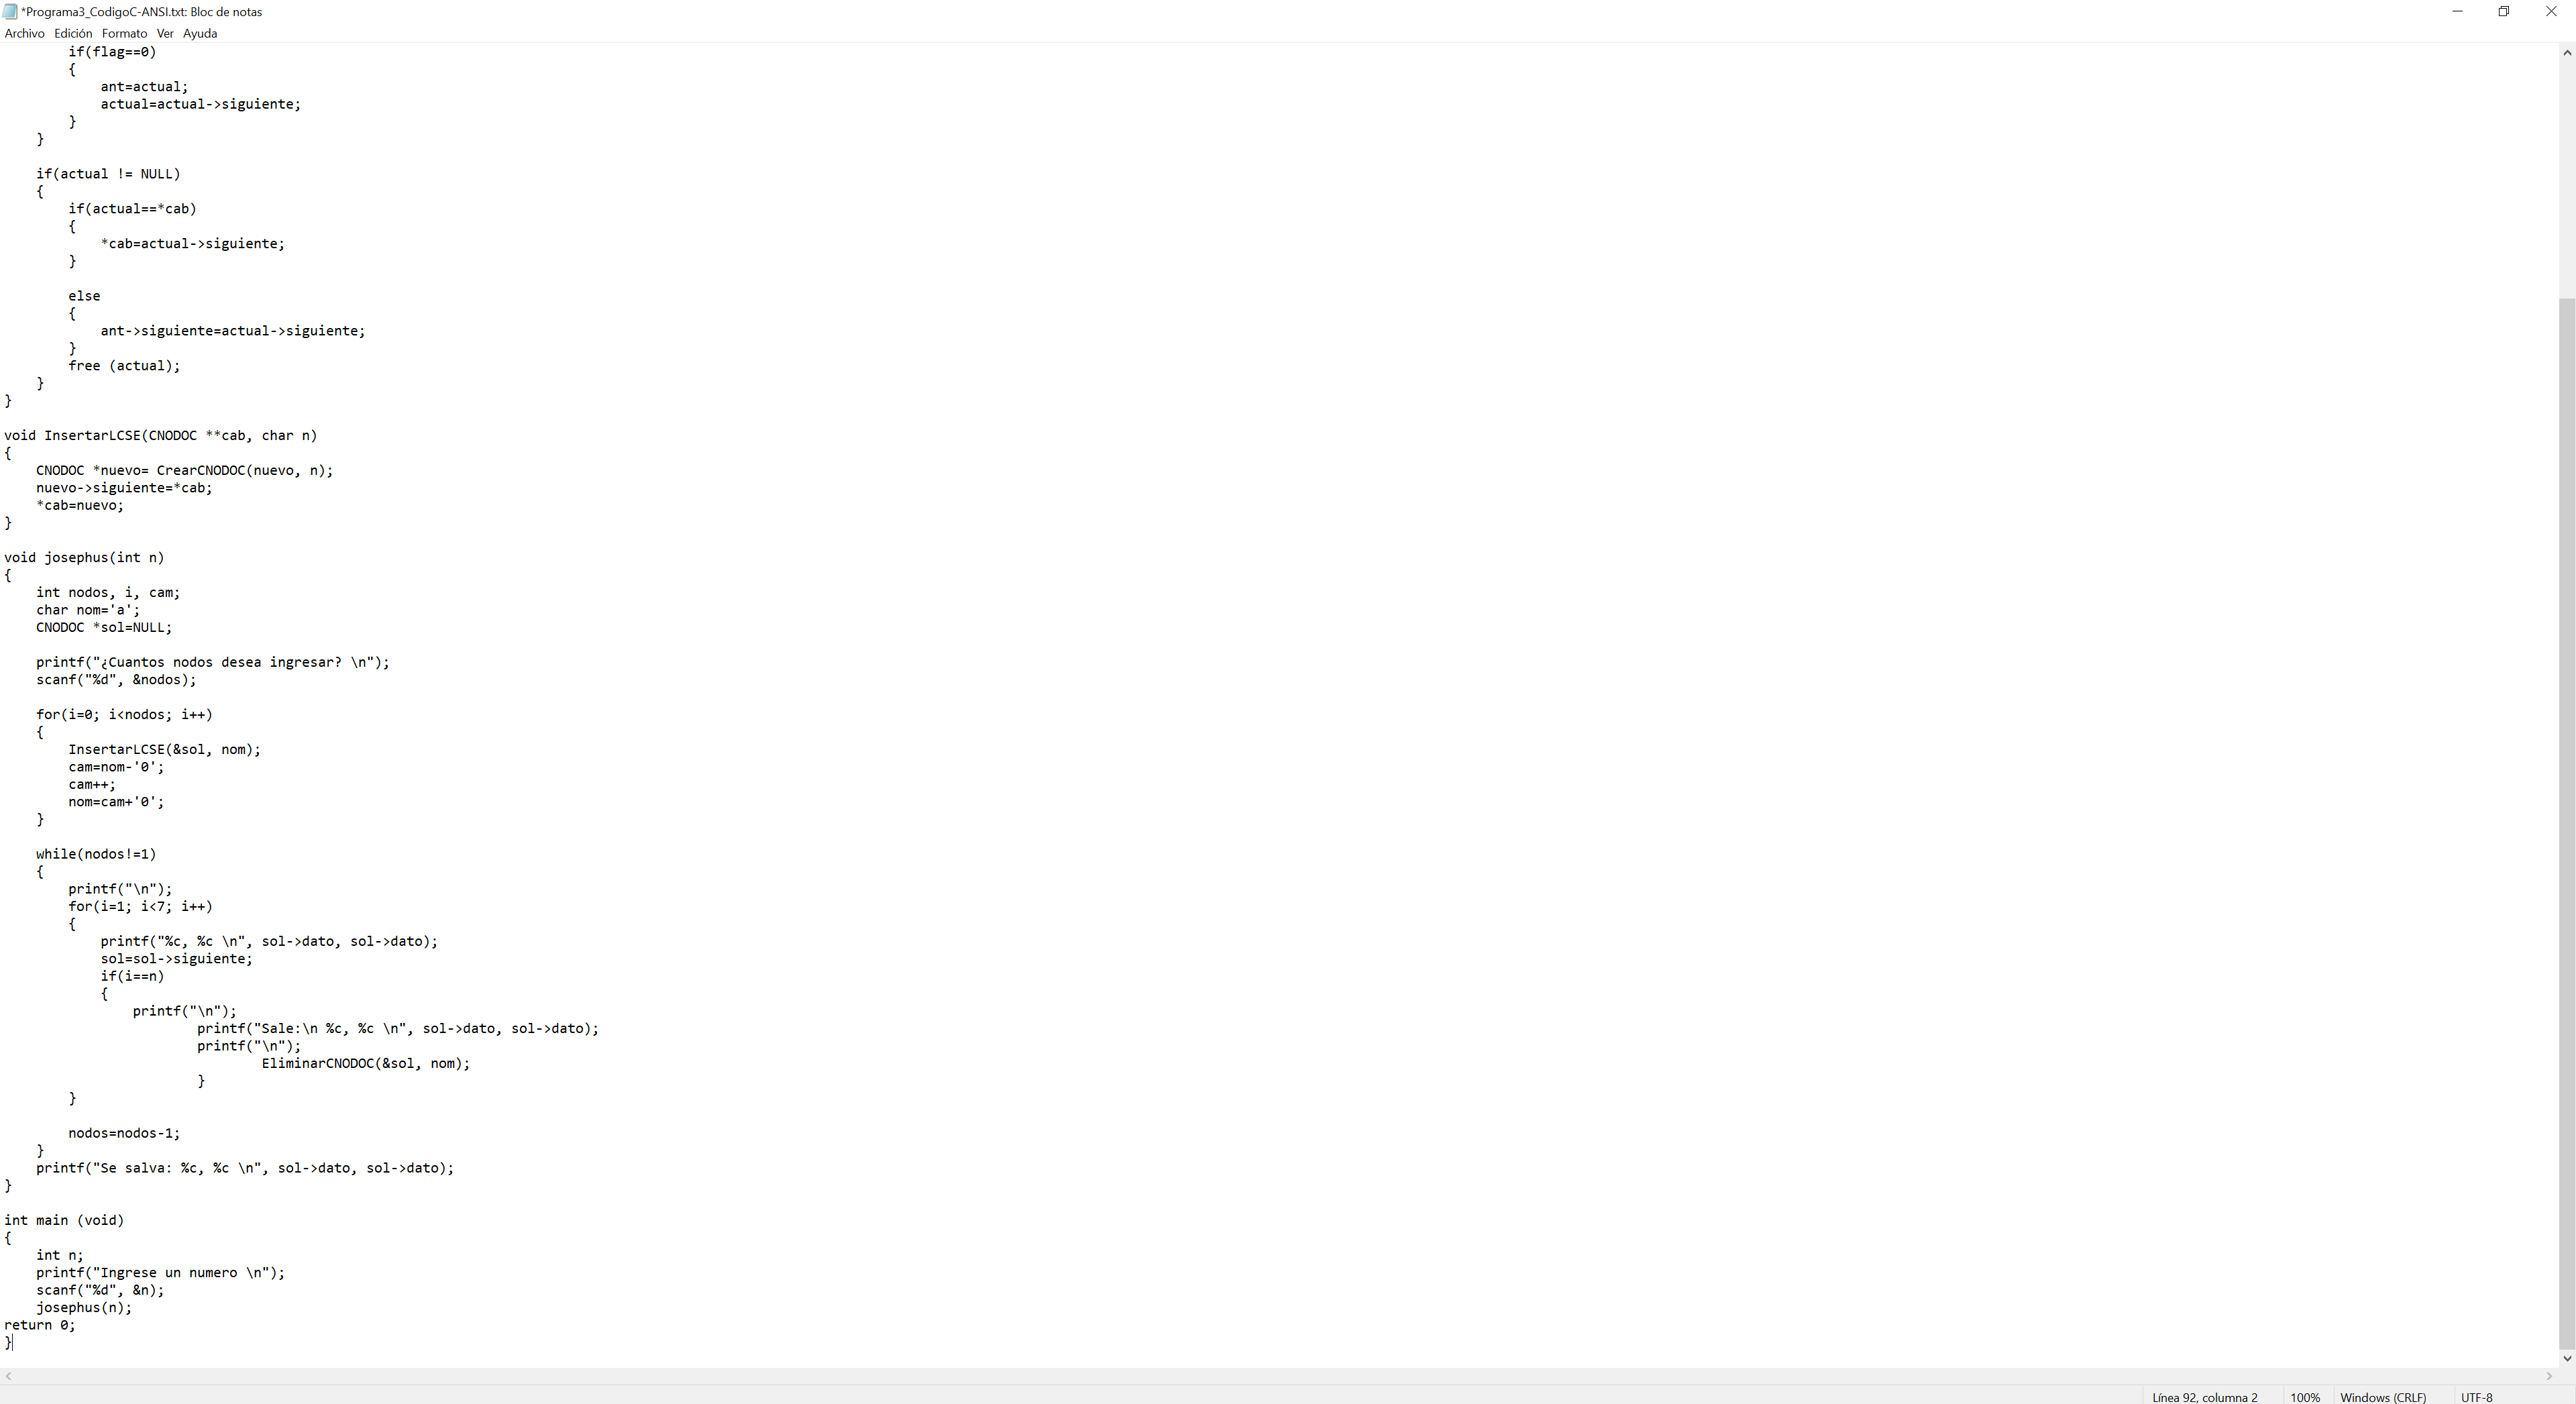
\includegraphics[width= 15cm, height= 5cm]{p3ar1.png}

Nos muestra cuanto encontro de cada palabra y el total
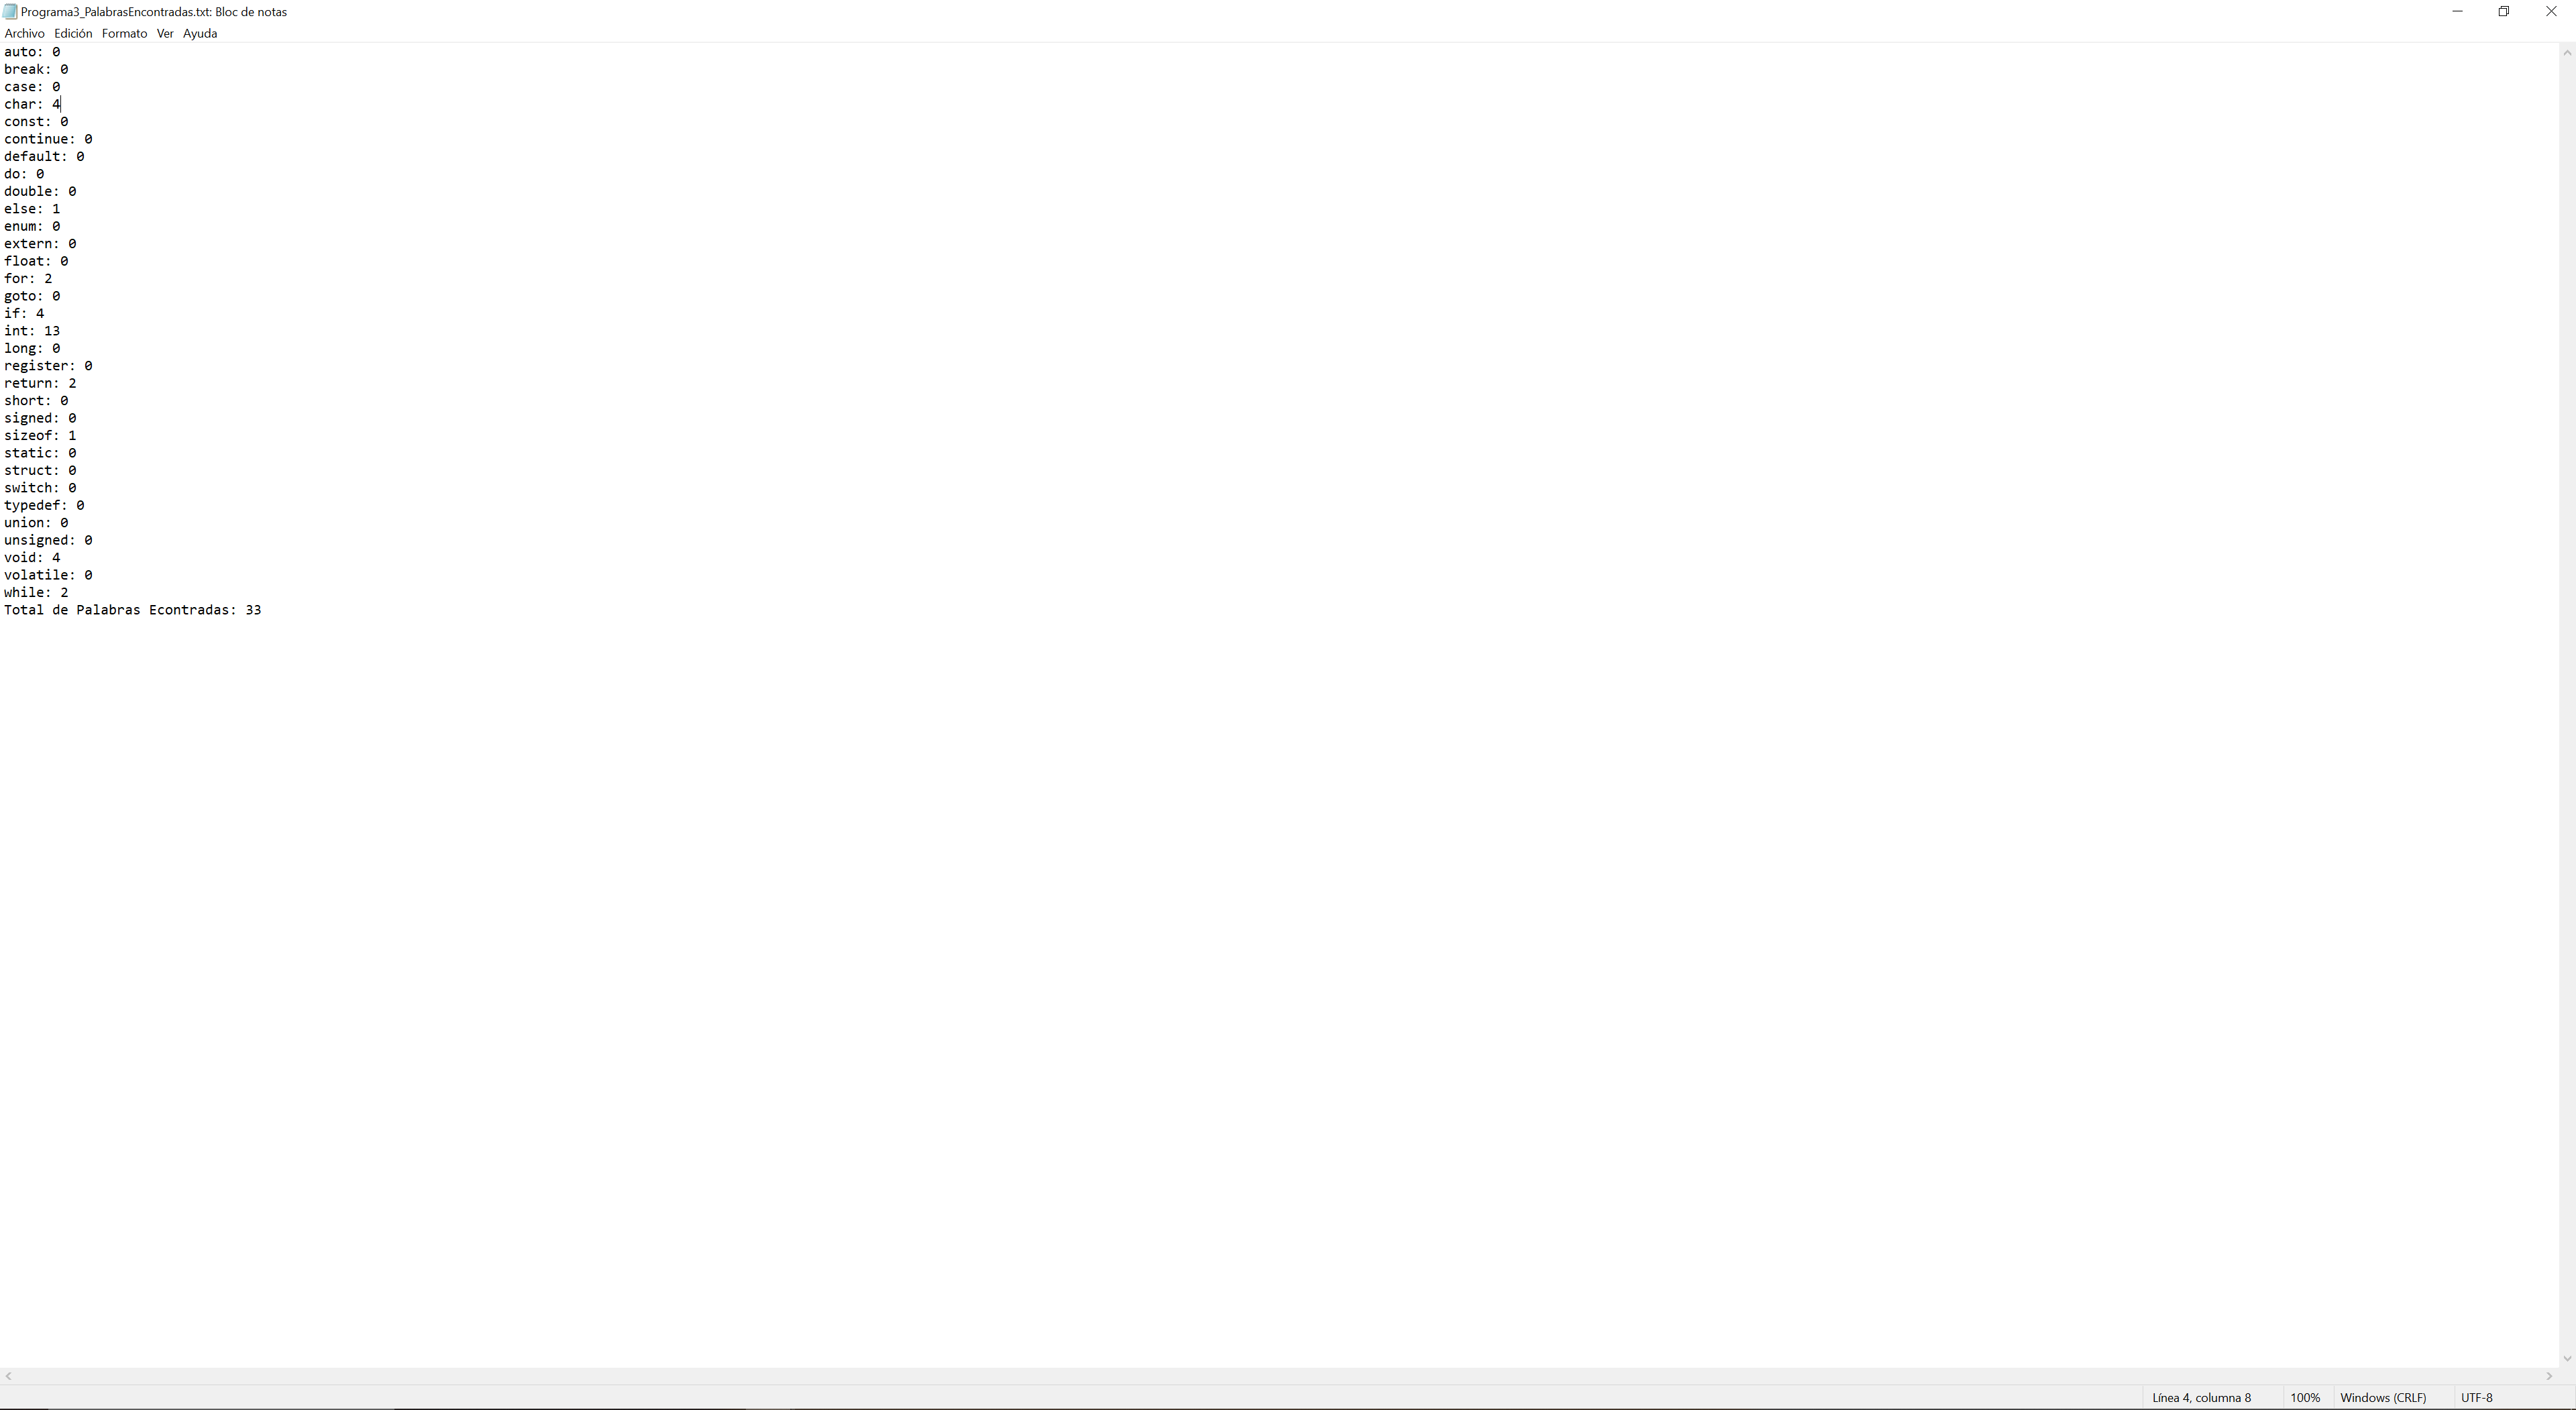
\includegraphics[width= 15cm, height= 5cm]{p3ar2.png}

Nos muestra los estados del automata
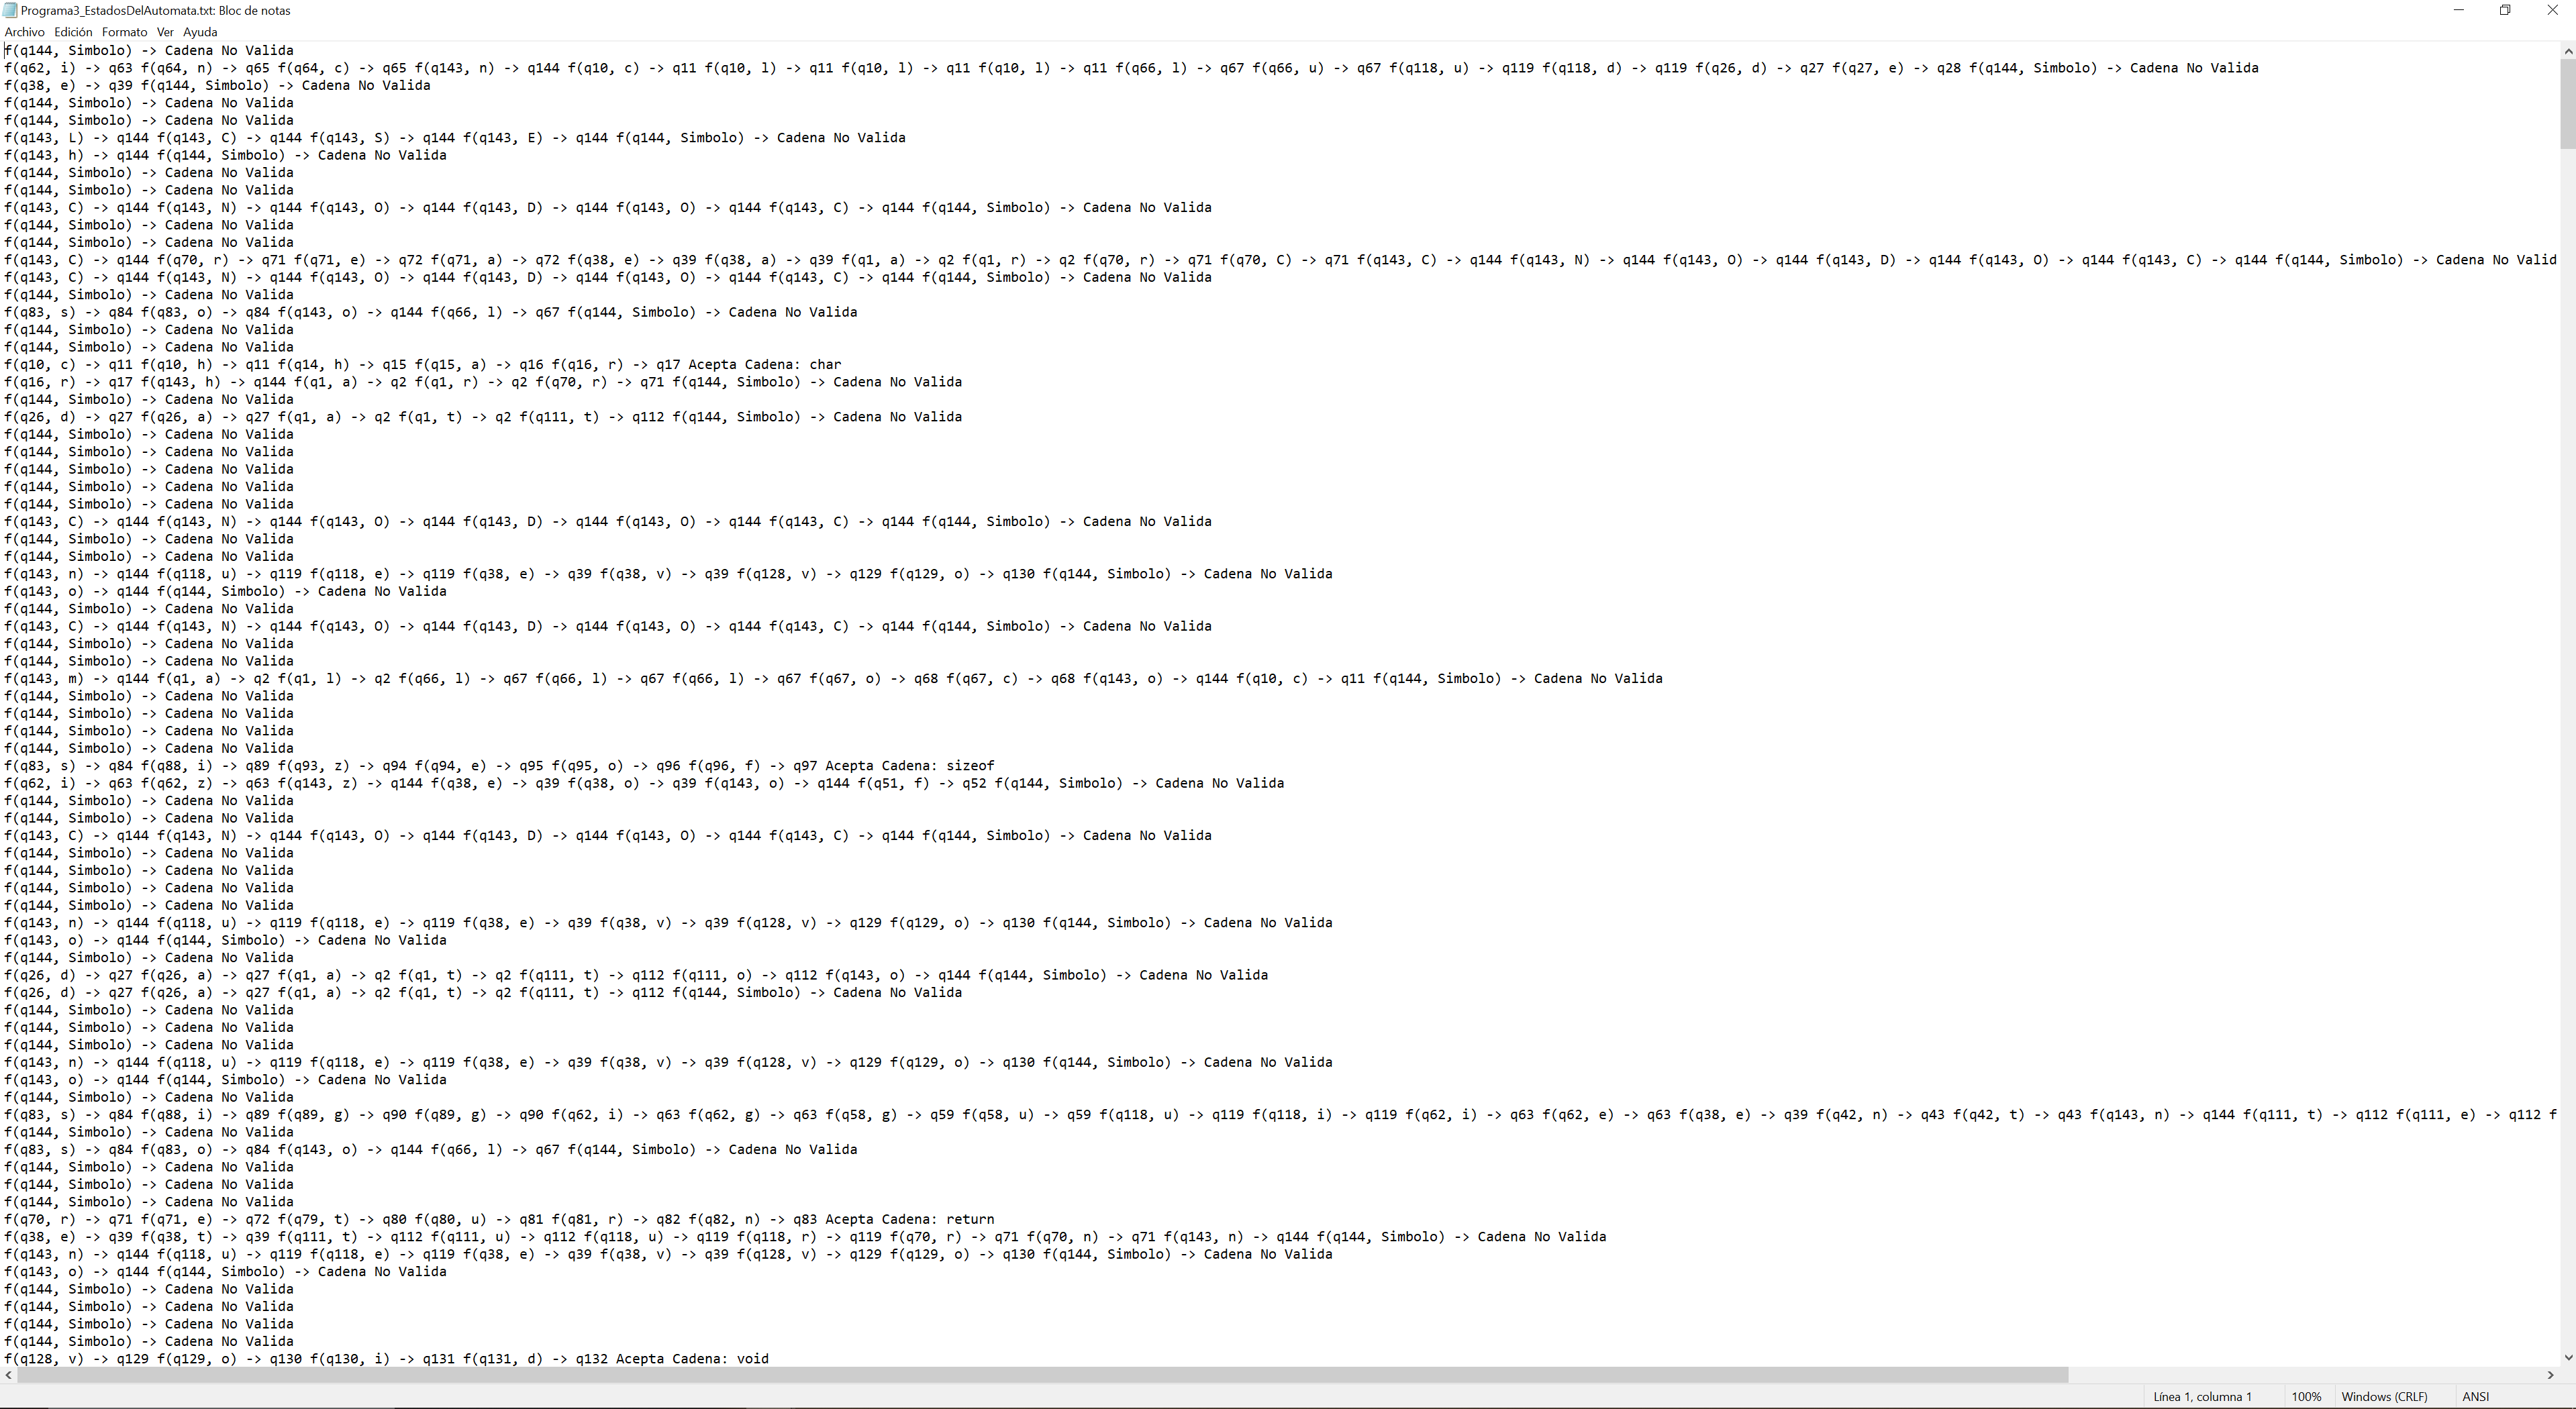
\includegraphics[width= 15cm, height= 5cm]{p3ar3.png}

Hubo un problema al quere graficar el grafo, no se encontro la forma de que el es vieran las letras dentro de cada uno de los nodos 
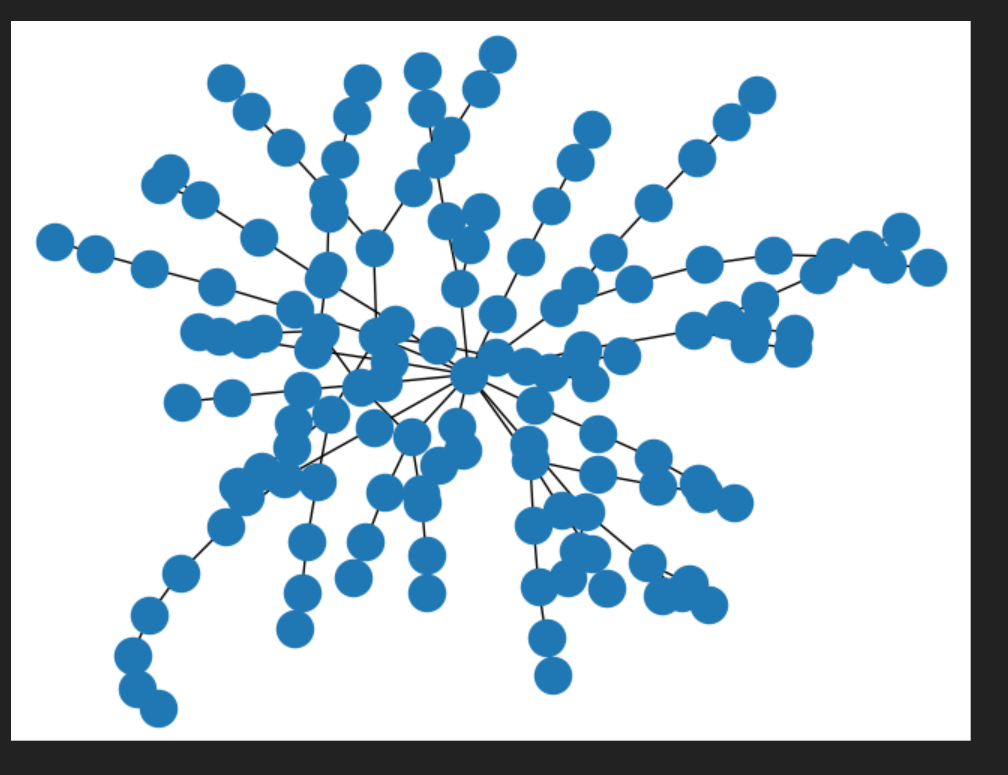
\includegraphics[width= 15cm, height= 5cm]{p3ar4.png}
\end{flushleft}
\end{document}